\documentclass{beamer}
\mode<presentation>{
  \usetheme{Boadilla}
  \usefonttheme[onlylarge]{structurebold}
  \usefonttheme[stillsansseriflarge]{serif}
  \setbeamerfont*{frametitle}{size=\normalsize,series=\bfseries}
  % \setbeamertemplate{navigation symbols}{}
  \setbeamercovered{transparent}
}
\usepackage[english]{babel}
\usepackage[latin1]{inputenc}
\usepackage{times}
\usepackage[T1]{fontenc}
\usepackage{amsmath}
\usepackage{amssymb}
\usepackage{esint}
\usepackage{hyperref}
\usepackage{tikz}
\usepackage{xkeyval}
\usepackage{xargs}
\usepackage{xcolor}
\usepackage{verbatim}
\usepackage{listings}
\usepackage{multimedia}
\usepackage{bm}
\usepackage{siunitx}
\usetikzlibrary{
  arrows,
  calc,
  decorations.pathmorphing,
  decorations.pathreplacing,
  decorations.markings,
  fadings,
  positioning,
  shapes,
  arrows.meta
}
\usepgfmodule{oo}

\pgfdeclareradialshading{glow2}{\pgfpoint{0cm}{0cm}}{
  color(0mm)=(white);
  color(2mm)=(white);
  color(8mm)=(black);
  color(10mm)=(black)
}
\pgfdeclareradialshading{glow}{\pgfpoint{0cm}{0cm}}{
  color(0mm)=(white);
  color(5mm)=(white);
  color(9mm)=(black);
  color(10mm)=(black)
}

\begin{tikzfadingfrompicture}[name=glow fading]
  \shade [shading=glow] (0,0) circle (1);
\end{tikzfadingfrompicture}

\begin{tikzfadingfrompicture}[name=glow2 fading]
  \shade [shading=glow2] (0,0) circle (1);
\end{tikzfadingfrompicture}

\mode<handout>{
  \usepackage{pgfpages}
  \pgfpagesuselayout{4 on 1}[a4paper,landscape,border shrink=5mm]
  \setbeamercolor{background canvas}{bg=black!10}
}

\newcommand\pgfmathsinandcos[3]{%
  \pgfmathsetmacro#1{sin(#3)}%
  \pgfmathsetmacro#2{cos(#3)}%
}
\newcommand\LongitudePlane[3][current plane]{%
  \pgfmathsinandcos\sinEl\cosEl{#2} % elevation
  \pgfmathsinandcos\sint\cost{#3} % azimuth
  \tikzset{#1/.estyle={cm={\cost,\sint*\sinEl,0,\cosEl,(0,0)}}}
}
\newcommand\LatitudePlane[3][current plane]{%
  \pgfmathsinandcos\sinEl\cosEl{#2} % elevation
  \pgfmathsinandcos\sint\cost{#3} % latitude
  \pgfmathsetmacro\yshift{\cosEl*\sint}
  \tikzset{#1/.estyle={cm={\cost,0,0,\cost*\sinEl,(0,\yshift)}}} %
}
\newcommand\DrawLongitudeCircle[2][1]{
  \LongitudePlane{\angEl}{#2}
  \tikzset{current plane/.prefix style={scale=#1}}
  % angle of "visibility"
  \pgfmathsetmacro\angVis{atan(sin(#2)*cos(\angEl)/sin(\angEl))} %
  \draw[current plane] (\angVis:1) arc (\angVis:\angVis+180:1);
  \draw[current plane,dashed] (\angVis-180:1) arc (\angVis-180:\angVis:1);
}
\newcommand\DrawLatitudeCircleArrow[2][1]{
  \LatitudePlane{\angEl}{#2}
  \tikzset{current plane/.prefix style={scale=#1}}
  \pgfmathsetmacro\sinVis{sin(#2)/cos(#2)*sin(\angEl)/cos(\angEl)}
  % angle of "visibility"
  \pgfmathsetmacro\angVis{asin(min(1,max(\sinVis,-1)))}
  \draw[current plane,decoration={markings, mark=at position 0.6 with {\arrow{<}}},postaction={decorate},line width=.6mm] (\angVis:1) arc (\angVis:-\angVis-180:1);
  \draw[current plane,dashed,line width=.6mm] (180-\angVis:1) arc (180-\angVis:\angVis:1);
}
\newcommand\DrawLatitudeCircle[2][1]{
  \LatitudePlane{\angEl}{#2}
  \tikzset{current plane/.prefix style={scale=#1}}
  \pgfmathsetmacro\sinVis{sin(#2)/cos(#2)*sin(\angEl)/cos(\angEl)}
  % angle of "visibility"
  \pgfmathsetmacro\angVis{asin(min(1,max(\sinVis,-1)))}
  \draw[current plane] (\angVis:1) arc (\angVis:-\angVis-180:1);
  \draw[current plane,dashed] (180-\angVis:1) arc (180-\angVis:\angVis:1);
}
\newcommand\coil[1]{
  {\rh * cos(\t * pi r)}, {\apart * (2 * #1 + \t) + \rv * sin(\t * pi r)}
}
\makeatletter
\define@key{DrawFromCenter}{style}[{->}]{
  \tikzset{DrawFromCenterPlane/.style={#1}}
}
\define@key{DrawFromCenter}{r}[1]{
  \def\@R{#1}
}
\define@key{DrawFromCenter}{center}[(0, 0)]{
  \def\@Center{#1}
}
\define@key{DrawFromCenter}{theta}[0]{
  \def\@Theta{#1}
}
\define@key{DrawFromCenter}{phi}[0]{
  \def\@Phi{#1}
}
\presetkeys{DrawFromCenter}{style, r, center, theta, phi}{}
\newcommand*\DrawFromCenter[1][]{
  \setkeys{DrawFromCenter}{#1}{
    \pgfmathsinandcos\sint\cost{\@Theta}
    \pgfmathsinandcos\sinp\cosp{\@Phi}
    \pgfmathsinandcos\sinA\cosA{\angEl}
    \pgfmathsetmacro\DX{\@R*\cost*\cosp}
    \pgfmathsetmacro\DY{\@R*(\cost*\sinp*\sinA+\sint*\cosA)}
    \draw[DrawFromCenterPlane] \@Center -- ++(\DX, \DY);
  }
}
\newcommand*\DrawFromCenterText[2][]{
  \setkeys{DrawFromCenter}{#1}{
    \pgfmathsinandcos\sint\cost{\@Theta}
    \pgfmathsinandcos\sinp\cosp{\@Phi}
    \pgfmathsinandcos\sinA\cosA{\angEl}
    \pgfmathsetmacro\DX{\@R*\cost*\cosp}
    \pgfmathsetmacro\DY{\@R*(\cost*\sinp*\sinA+\sint*\cosA)}
    \draw[DrawFromCenterPlane] \@Center -- ++(\DX, \DY) node {#2};
  }
}
\makeatother

% not mandatory, but I though it was better to set it blank
\setbeamertemplate{headline}{}
\def\beamer@entrycode{\vspace{-\headheight}}

\tikzstyle{snakearrow} = [decorate, decoration={pre length=0.2cm,
  post length=0.2cm, snake, amplitude=.4mm,
  segment length=2mm},thick, ->]

%% document-wide tikz options and styles

\tikzset{%
  % >=latex, % option for nice arrows
  inner sep=0pt,%
  outer sep=2pt,%
  mark coordinate/.style={inner sep=0pt,outer sep=0pt,minimum size=3pt,
    fill=black,circle}%
}
\tikzset{
  % Define standard arrow tip
  >=stealth',
  % Define style for boxes
  punkt/.style={
    rectangle,
    rounded corners,
    draw=black, very thick,
    text width=8em,
    minimum height=2.5em,
    text centered},
}

\tikzset{onslide/.code args={<#1>#2}{%
    \only<#1>{\pgfkeysalso{#2}}
    % \pgfkeysalso doesn't change the path
  }}
\tikzset{alt/.code args={<#1>#2#3}{%
    \alt<#1>{\pgfkeysalso{#2}}{\pgfkeysalso{#3}}
    % \pgfkeysalso doesn't change the path
  }}
\tikzset{temporal/.code args={<#1>#2#3#4}{%
    \temporal<#1>{\pgfkeysalso{#2}}{\pgfkeysalso{#3}}{\pgfkeysalso{#4}}
    % \pgfkeysalso doesn't change the path
  }}

\makeatletter
\newbox\@backgroundblock
\newenvironment{backgroundblock}[2]{%
  \global\setbox\@backgroundblock=\vbox\bgroup%
  \unvbox\@backgroundblock%
  \vbox to0pt\bgroup\vskip#2\hbox to0pt\bgroup\hskip#1\relax%
}{\egroup\egroup\egroup}
\addtobeamertemplate{background}{\box\@backgroundblock}{}
\makeatother

% \def\timeleft{15:00->14:55}

\title[Interaction between single atoms]{Interaction between single atoms\\in optical tweezers}
\date{May 29, 2019}
\author[Yichao Yu]{Yichao Yu\\
  \vspace{0.5cm}
  {\footnotesize Lee Liu, Kenneth Wang, Lewis Picard, Jonathan Hood}\\
  {\footnotesize Jessie T. Zhang, Eliot Fenton, Yen-Wei Lin}}
\institute{Ni Group/Harvard}

\begin{document}

\pgfdeclarelayer{tweezer}
\pgfsetlayers{tweezer,main}
\pgfooclass{tweezer}{
  \method tweezer() {
  }
  \method drawTweezer(#1,#2,#3) {
    \begin{pgfonlayer}{tweezer}
      \shade[shading=radial,path fading=glow fading,shift={(#1,#2)},rotate=90,yscale=1,
      fill opacity=0.9,inner color=#3]
      plot[draw,samples=200,domain=-1.5:1.5] function {sqrt(0.01 + x**2 / 5)}
      -- plot[draw,samples=200,domain=1.5:-1.5] function {-sqrt(0.01 + x**2 / 5)};
    \end{pgfonlayer}
  }
  \method drawAtom(#1,#2,#3,#4) {
    \fill [#4,path fading=glow2 fading] (#1,#2) circle (#3);
  }
  \method drawNaAtom(#1,#2,#3) {
    \pgfoothis.drawAtom(#1,#2,#3,orange);
  }
  \method drawCsAtom(#1,#2,#3) {
    \pgfoothis.drawAtom(#1,#2,#3,blue);
  }
  \method drawNaTweezer(#1,#2) {
    \pgfoothis.drawTweezer(#1,#2,orange!35!black!30);
  }
  \method drawCsTweezer(#1,#2) {
    \pgfoothis.drawTweezer(#1,#2,blue!30!black!30);
  }
  \method up(#1,#2) {
    \pgfoothis.drawCsTweezer(#1,#2);
    \pgfoothis.drawNaAtom(#1,#2+0.06,0.12);
    \pgfoothis.drawCsAtom(#1,#2-0.06,0.16);
  }
  \method down(#1,#2) {
    \pgfoothis.drawCsTweezer(#1,#2);
    \pgfoothis.drawCsAtom(#1,#2+0.06,0.16);
    \pgfoothis.drawNaAtom(#1,#2-0.06,0.12);
  }
  \method naTrap(#1,#2) {
    \pgfoothis.drawNaTweezer(#1,#2);
    \pgfoothis.drawNaAtom(#1,#2,0.12);
  }
  \method csTrap(#1,#2) {
    \pgfoothis.drawCsTweezer(#1,#2);
    \pgfoothis.drawCsAtom(#1,#2,0.16);
  }
}
\pgfoonew \mytweezer=new tweezer()

% Title
%% You've heard Jessie's talk about our experiment on ????.
%% Now I'll talk about some other experiments we've done
%% on the interactions between two atoms in optical tweezers
%% that are not directly making molecules.
%% These experiements are done to improve our understanding of the molecule
%% and to help with our molecule formation process.

{
  \usebackgroundtemplate{
    \makebox[\paperwidth][c]{\centering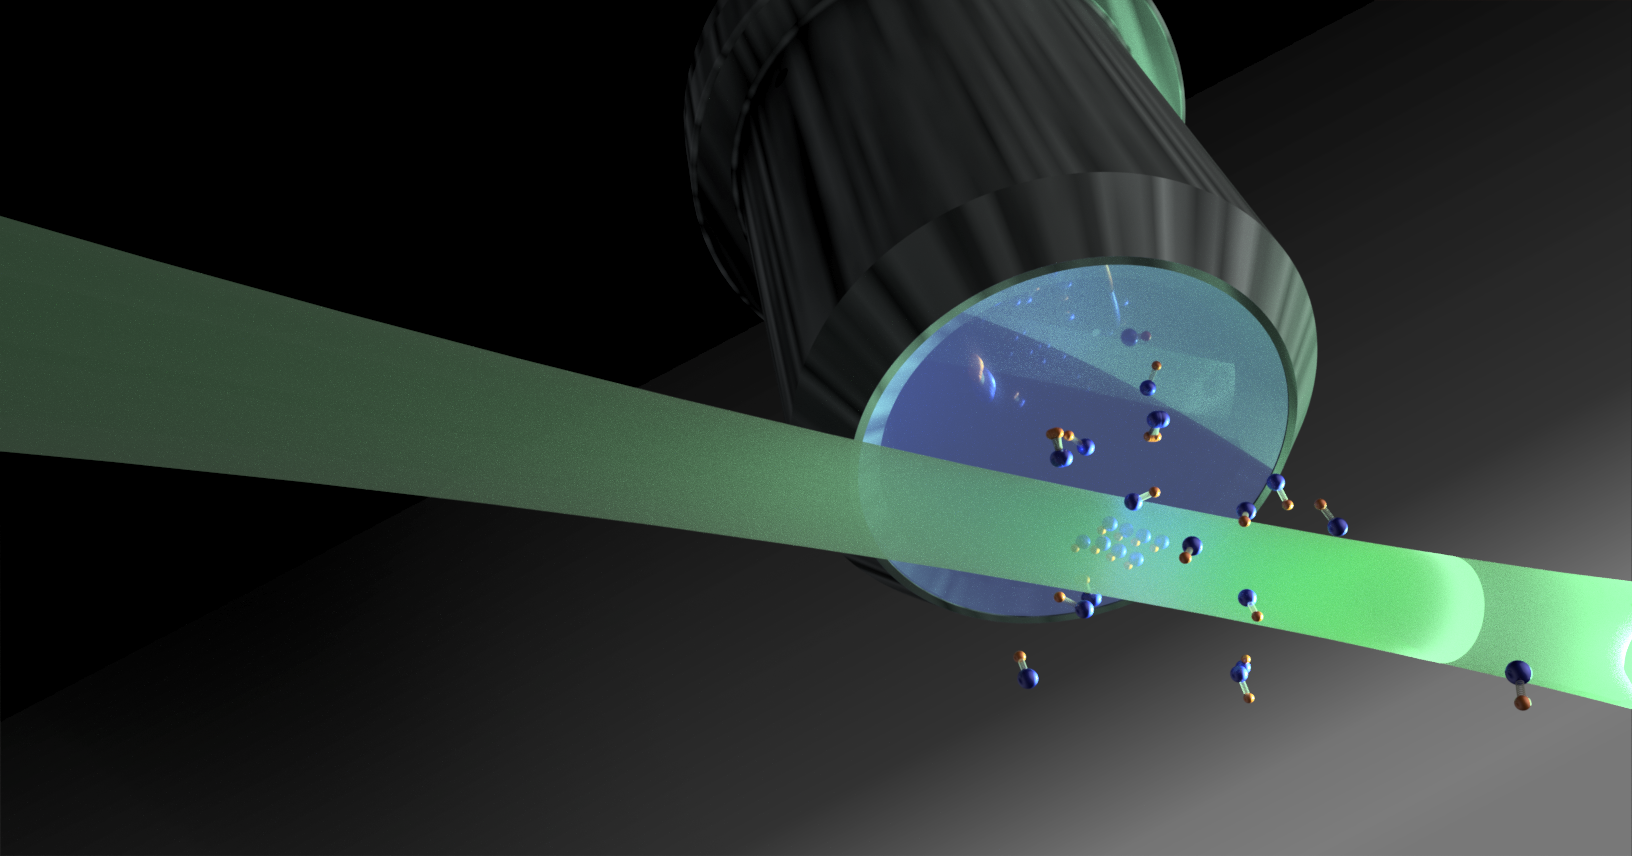
\includegraphics[width=\paperwidth]{front_bg.png}}
  }
  \setbeamercolor{title}{fg=white}
  \setbeamercolor{author}{fg=white}
  \setbeamercolor{institute}{fg=white}
  \setbeamercolor{date}{fg=white}
  \begin{frame}{}
    \titlepage
  \end{frame}
}

% All of our experiments are done on single Na and Cs atoms in an optical tweezer.
%% * Start with single atoms (Na and Cs) trapped from laser cooled gas
%% * RSC and OP to prepare a single quantum state
%% * Merge to enable interaction
\begin{frame}[t]{}
  \begin{center}
    \begin{tikzpicture}[scale=0.75]
      \mytweezer.drawCsTweezer(0, 0)
      \mytweezer.drawNaTweezer(-1, 0)
      \mytweezer.drawCsAtom(-0.07, 0.08, 0.22)
      \mytweezer.drawNaAtom(-1.06, -0.09, 0.27)

      \mytweezer.drawCsTweezer(0, -3.1)
      \mytweezer.drawNaTweezer(-1, -3.1)
      \mytweezer.drawCsAtom(0.0, -3.1, 0.12)
      \mytweezer.drawNaAtom(-1.0, -3.1, 0.16)

      \mytweezer.drawCsTweezer(-1, -7.0)
      \mytweezer.drawNaAtom(-1.05, -6.87, 0.16)
      \mytweezer.drawCsAtom(-0.95, -7.13, 0.12)

      \fill[white,temporal=<1>{opacity=0.82}{opacity=0}{opacity=0.5}]
      (-1.5, 1.5) rectangle (0.5, -1.5);
      \fill[white,temporal=<2>{opacity=0.82}{opacity=0}{opacity=0.5}]
      (-1.5, 1.5 - 3.1) rectangle (0.5, -1.5 - 3.1);
      \fill[white,temporal=<3>{opacity=0.82}{opacity=0}{opacity=0.5}]
      (-1.5, 1.5 - 7.0) rectangle (-0.5, -1.5 - 7.0);

      \visible<2->{
        \begin{scope}[alt=<2>{opacity=0.7}{opacity=0.35}]
          \draw[orange,dotted,line width=1.2] (-1, -0.4) -- (-1, -2.9);
          \draw[blue,dotted,line width=1.2] (0, -0.15) -- (0, -2.9);
        \end{scope}
      }

      \visible<3->{
        \begin{scope}[alt=<3>{opacity=0.7}{opacity=0.35}]
          \draw[->,orange,line width=1.2] (-1, -3.3) -- (-1, -6.7);
          \draw[->,blue,domain=-3.3:-6.7,smooth,variable=\y,line width=1.2]
          plot ({atan((\y+4.7) * 5) / 170 - 0.5},{\y});
        \end{scope}
      }
      \visible<1>{
        \node[above,align=center] at (7, 0)
        {\usebeamerfont{frametitle}\usebeamercolor[fg]{frametitle}{\Large Loading}};
        \node[below,align=center] at (6.5, -0.5)
        {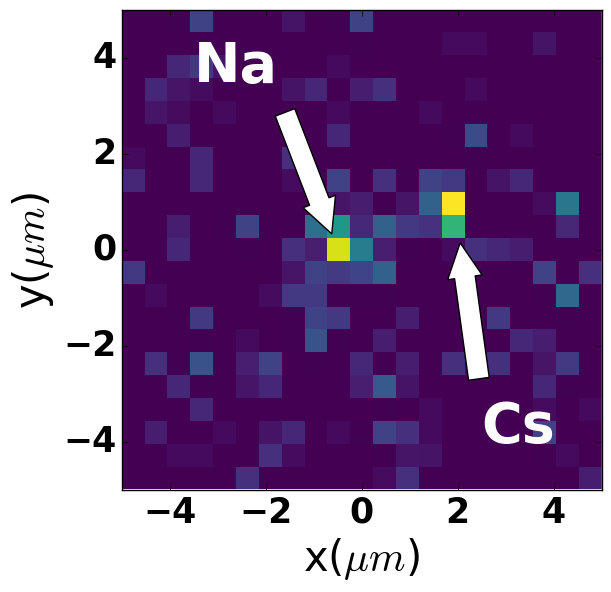
\includegraphics[width=5cm]{../../experiments/nacs_atoms/imgs/single_viridis.png}};
        \node[below,align=center] at (7, -7.5)
        {Loading probability per site: 60\%\\
          Post select on initial and final state.};
      }
      \visible<2>{
        \node[above,align=center] at (7, 0)
        {\usebeamerfont{frametitle}\usebeamercolor[fg]{frametitle}{\Large Cooling}};
        \node[below] at (6.5, -1)
        {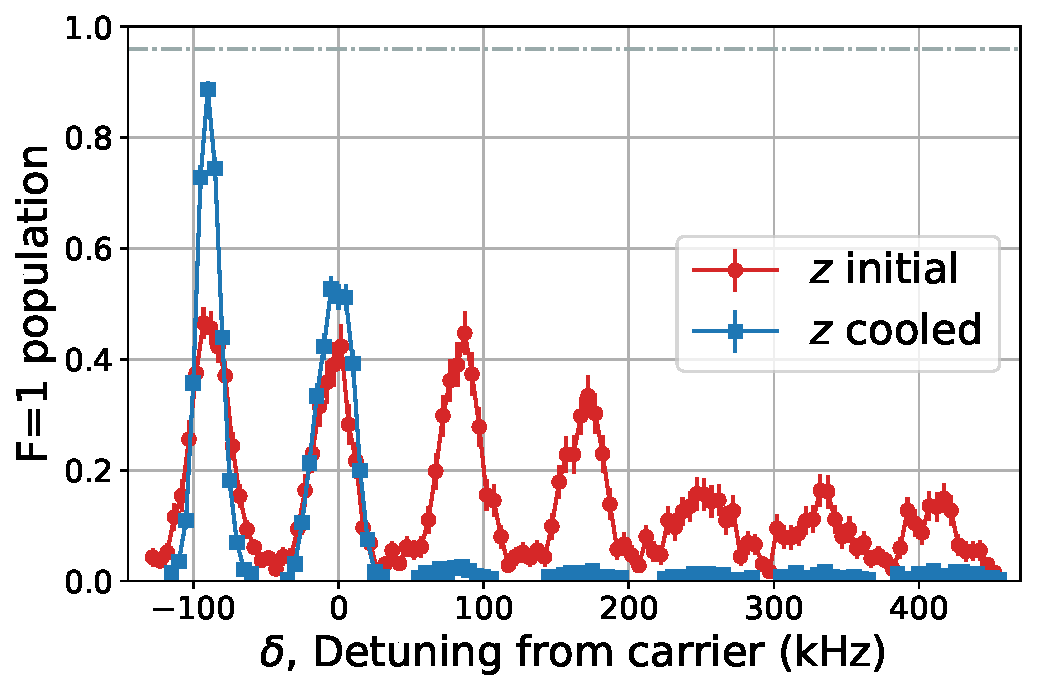
\includegraphics[width=6cm]{spectrum_nolabel_az.pdf}};
        Don't mention axis.
        Explain the sideband spectrum more.
        \only<2>{
          \node[below,align=center] at (7, -7)
          {Cs: 96\% ground state\footnote{Phys. Rev. X 9, 021039}\\
            Na: 94\% ground state\footnote{Phys. Rev. A 97, 063423}};
        }
      }
      \visible<3>{
        \node[above,align=center] at (7, 0)
        {\usebeamerfont{frametitle}\usebeamercolor[fg]{frametitle}{\Large Merging}};
        \draw[orange,line width=1.5] plot[draw,samples=200,domain=4.5:10.5]
        function {-0.22 * exp(-(x - 9)**2 / 0.75**2) + -0.4 * exp(-(x - 6)**2 / 0.75**2) - 1};
        \draw[blue,line width=1.5] plot[draw,samples=200,domain=4.5:10.5]
        function {-1.2 * exp(-(x - 9)**2 / 0.75**2) + 0.45 * exp(-(x - 6)**2 / 0.75**2) - 1};
        \mytweezer.drawNaAtom(6, -1.22, 0.15)
        \mytweezer.drawCsAtom(9, -2.06, 0.11)

        \draw[orange,line width=1.5] plot[draw,samples=200,domain=4.5:10]
        function {-0.22 * exp(-(x - 7.5)**2 / 0.75**2) + -0.4 * exp(-(x - 6)**2 / 0.75**2) - 3.5};
        \draw[blue,line width=1.5] plot[draw,samples=200,domain=4.5:10]
        function {-1.2 * exp(-(x - 7.5)**2 / 0.75**2) + 0.45 * exp(-(x - 6)**2 / 0.75**2) - 3.5};
        \mytweezer.drawNaAtom(6, -3.72, 0.15)
        \mytweezer.drawCsAtom(7.5, -4.56, 0.11)

        \draw[orange,line width=1.5] plot[draw,samples=200,domain=4.5:8.5]
        function {-0.22 * exp(-(x - 6)**2 / 0.75**2) + -0.4 * exp(-(x - 6)**2 / 0.75**2) - 6};
        \draw[blue,line width=1.5] plot[draw,samples=200,domain=4.5:8.5]
        function {-1.2 * exp(-(x - 6)**2 / 0.75**2) + 0.45 * exp(-(x - 6)**2 / 0.75**2) - 6};
        \mytweezer.drawNaAtom(5.9, -6.42, 0.12)
        \mytweezer.drawCsAtom(6.05, -6.6, 0.13)

        \draw[orange,line width=1.5] plot[draw,samples=200,domain=4.5:8.5]
        function {-0.22 * exp(-(x - 6)**2 / 0.75**2) - 8.5};
        \draw[blue,line width=1.5] plot[draw,samples=200,domain=4.5:8.5]
        function {-1.2 * exp(-(x - 6)**2 / 0.75**2) - 8.5};
        \mytweezer.drawNaAtom(6, -8.55, 0.14)
        \mytweezer.drawCsAtom(6, -9.56, 0.11)

        \draw[dotted,line width=2,black!30,opacity=10] (0.3, -3.0) -- (4.5, -0.5);
        \draw[dotted,line width=2,black!30,opacity=10] (-0.7, -7.0) -- (4.5, -9.3);
      }
    \end{tikzpicture}
    \vspace{-2cm}
  \end{center}
\end{frame}

% One measurement we can do is the scattering length
%% between Na and Cs since it captures many aspects of the atom-atom interaction
%% * Binding energy
%% * Molecular potential
%% * Feshbach resonance
%% * Molecule formation
\begin{frame}{Scattering length $a$}
  \begin{columns}
    \column{4.5cm}
    \begin{itemize}
    \item<2-> Binding energy
    \item<3-> Molecular potential
    \item<4-> Feshbach resonance
    \item<5-> Molecule formation\\
      $\vdots$
    \end{itemize}
    \column{6.5cm}
    \begin{tikzpicture}
      \begin{scope}[scale=0.65]
        \draw[->,line width=1.2] (0, 0) -- (0, 8);
        \node[above,rotate=90] at (0, 4) {Energy};
        \draw[->,line width=1.2] (0, 0) -- (8, 0);
        \node[below] at (4, -0.5) {Internuclear distance};

        \draw[dashed] (1.0269 - 0.25, 2.5) -- (7 - 0.25, 2.5);
        \draw (1.0793 - 0.25, -0.4631 + 2.5) -- (4.5 - 0.25, -0.4631 + 2.5);

        \draw[line width=1.1]
        plot[samples=200,domain=0.8:7,variable=\x]
        ({\x - 0.25}, {6.8*\x^(-3.4)-6.5*\x^(-1.7) + 2.5});

        \mytweezer.drawNaAtom(5.55, 2.7, 0.12)
        \mytweezer.drawCsAtom(6.05, 2.7, 0.10)

        \mytweezer.drawNaAtom(2.08, 2.15, 0.12)
        \mytweezer.drawCsAtom(2.25, 2.15, 0.10)

        \draw[->, cyan!50!blue, line width=0.8] (5.4, 2.7) -- ++(-3.5, 0)
        arc (270:90:0.2) -- ++(2.5, 0);
      \end{scope}
    \end{tikzpicture}
  \end{columns}
\end{frame}

%% We measure the scattering length using interaction shift.
%% When we successfully loaded two atoms in the tweezer,
%% their energy levels will be shifted due to the interaction.
%% This shift depends on the spin state of the atom and we can measure this difference
%% by driving a Raman or microwave transition between HF states.
%% As shown.... by comparing the spectrum with and without another atom...
%% This way of measuring the scattering length is similar to the experiement done
%% in optical lattice on Mott insulator but the anisotropy causes some difference as shown in.

% Interaction shift data
%% One peak on the right, lowering energy -> attractive interaction.
%% Another peak on the left...
%% Significant state mixing due to low axial trapping frequency
%% Theory model
%% 33+22 -> 33+11

\begin{frame}{Interaction shift}
  \vspace{-0.8cm}
  \begin{tikzpicture}
    \draw[white,opacity=0] (-6, -4.5) rectangle (6, 4.5);
    % Raman sequence
    \visible<1>{
      \node at (-2.8, 0.7) {\includegraphics[width=6cm]{shift_raman_1.pdf}};
    }
    \visible<2-3>{
      \node at (-2.8, 0.7) {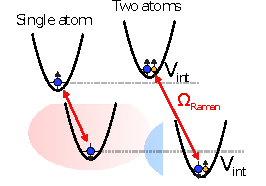
\includegraphics[width=6cm]{shift_raman.pdf}};
    }
    % Data 1
    \visible<3-6>{\node at (3.2, 0) {\includegraphics[width=5cm]{na2cs4_0.pdf}};}
    \visible<7>{\node at (3.2, 0) {\includegraphics[width=5cm]{na2cs4.pdf}};}
    \visible<8->{\node at (3.2, 0) {\includegraphics[width=5cm]{na2cs3.pdf}};}

    % Equations
    \visible<4-5>{
      \node[below right,align=left] at (-4.9, 3.8)
      {\footnotesize $\displaystyle H=\!\!\sum_{i=x,y,z}(\frac{m_{1}\omega_{1,i}^2x_{1,i}^2}{2}+\frac{p_{1,i}^2}{2m_{1}})\ +\!\sum_{i=x,y,z}(\frac{m_{2}\omega_{2,i}^2x_{2,i}^2}{2}+\frac{p_{2,i}^2}{2m_{2}})+V_{int}(\vec r_1-\vec r_2)$};
      \draw[decoration={brace,mirror,amplitude=10pt},decorate,line width=1]
      (-4.15,2.8) -- node[below=10pt] {\small Na} (-1.15,2.8);
      \draw[decoration={brace,mirror,amplitude=10pt},decorate,line width=1]
      (-0.5,2.8) -- node[below=10pt] {\small Cs} (2.5,2.8);
      \draw[decoration={brace,mirror,amplitude=10pt},decorate,line width=1]
      (3.05,3) -- node[below=10pt] {\small Interaction} (4.55,3);
    }
    \visible<5>{
      \node[above right,align=left] at (-5.8, -2.3)
      {
        \textcolor{blue!60!black}{To center of mass}\\
        \textcolor{blue!60!black}{and relative coordinates}\\
        \\
        {\tiny
          $\begin{aligned}
            M=&\ m_1+m_2&\mu=&\ \frac{m_1m_2}{m_1+m_2}\\
            \Omega_i^2=&\ \frac{m_1\omega_{1,i}^2+m_2\omega_{2,i}^2}{m_1+m_2}&\omega_{R,i}^2=&\ \frac{m_2\omega_{1,i}^2+m_1\omega_{2,i}^2}{m_1+m_2}\\
            X_i=&\ \frac{m_1x_{1,i}+m_2x_{2,i}}{m_1+m_2}&x_{R,i}=&\ x_{1,i}-x_{2,i}\\
            P_i=&\ p_{1,i}+p_{2,i}&p_{R,i}=&\ \frac{m_2p_{1,i}-m_1p_{2,i}}{m_1+m_2}
          \end{aligned}$}};
    }
    \visible<5->{
      \node[above right,align=left] at (-6, -4.5)
      {\footnotesize $\displaystyle H=\!\!\sum_{i=x,y,z}(\frac{M\Omega_{i}^2X_{i}^2}{2}+\frac{P_{i}^2}{2M})\ +\!\sum_{i=x,y,z}(\frac{\mu\omega_{R,i}^2x_{R,i}^2}{2}+\frac{p_{R,i}^2}{2\mu})+V_{int}(\vec r_R)\ +\!\sum_{i=x,y,z}\mu(\omega_{1,i}^2 - \omega_{2,i}^2)X_ix_{R,i}$};
      \draw[decoration={brace,amplitude=10pt},decorate,line width=1]
      (-5.25,-3.5) -- node[above=10pt] {\small Center of mass} (-2.5,-3.5);
      \draw[decoration={brace,amplitude=10pt},decorate,line width=1]
      (-1.9,-3.5) -- node[above=10pt] {\small Relative} (2.4,-3.5);
      \draw[decoration={brace,amplitude=10pt},decorate,line width=1]
      (3,-3.5) -- node[above=10pt] {\small Mixing} (5.9,-3.5);
    }
    \visible<6>{
      \node at (-2.6, 0.5) {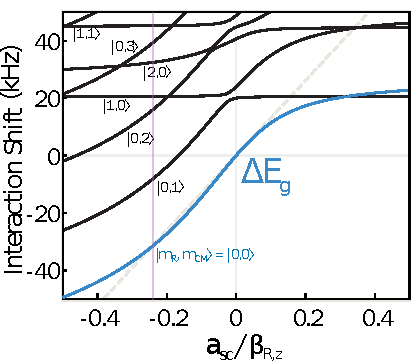
\includegraphics[width=6cm]{shift_theory.pdf}};
    }
    \visible<7>{
      \node at (-2.6, 0.5) {\includegraphics[width=6cm]{shift_theory42_32.pdf}};
    }
    \visible<8->{
      \node at (-2.6, 0.5) {\includegraphics[width=6cm]{shift_theory32_31.pdf}};
    }
    \visible<9->{
      \fill[white,opacity=0.95] (-6, -4.5) rectangle (6, 3.5);
      \node[align=center] at (0, 2.1)
      {Combined with binding energy measurement on Na(2,2) Cs(4,4)\\
        \\
        \begin{tabular}{|c|c|}
          \hline
          Spin state ($F,m_F$)&Scattering length (a.u.)\\\hline
          Na(2,2) Cs(4,4)&30.36\\\hline
          Na(2,2) Cs(3,3)&-693.8\\\hline
          Na(1,1) Cs(3,3)&13.19\\\hline
        \end{tabular}};
    }
    \visible<10->{
      \draw[->, line width=1, color=red!50!black] (0.8, 1.45) -- (-2, 0.5)
      node[below] {Enhanced coupling to molecular state?};
    }
    \visible<11->{
      \node at (1.3, -2) {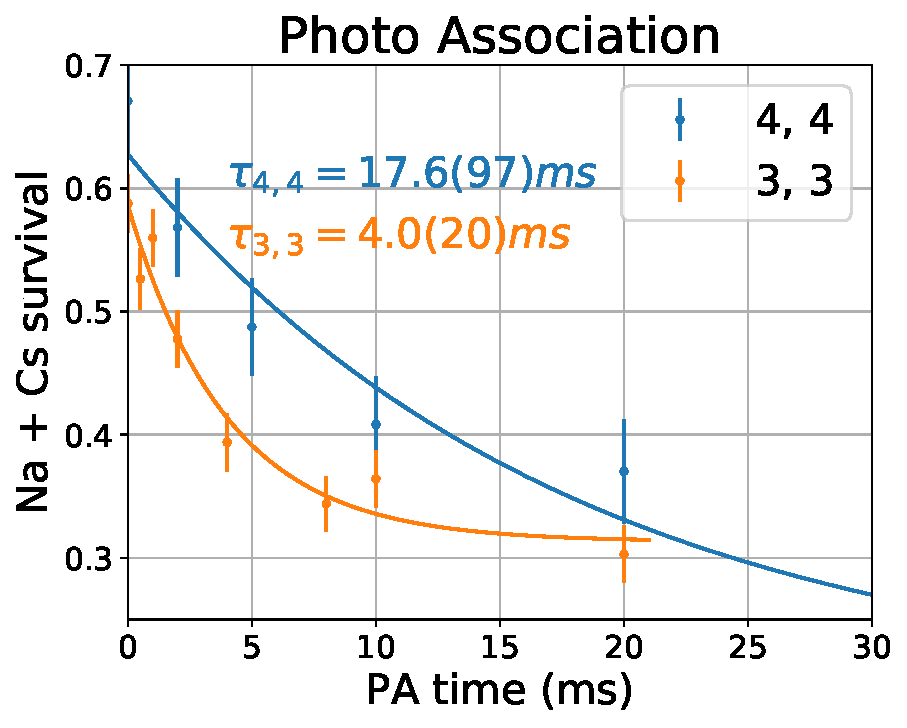
\includegraphics[width=5cm]{../../experiments/nacs_201904/imgs/data_20190521_lifetime_cmp_lin.pdf}};
    }
  \end{tikzpicture}
\end{frame}

% Another thing we can measure is the FB resonance
%% Better prediction than before.
\begin{frame}[t]{Na (1, -1) Cs (3, -3) Feshbach resonance}
  \only<1>{
    \begin{center}
      \includegraphics[height=7cm]{chamber1_5.jpg}
    \end{center}
  }
  \only<2->{
    \begin{center}
      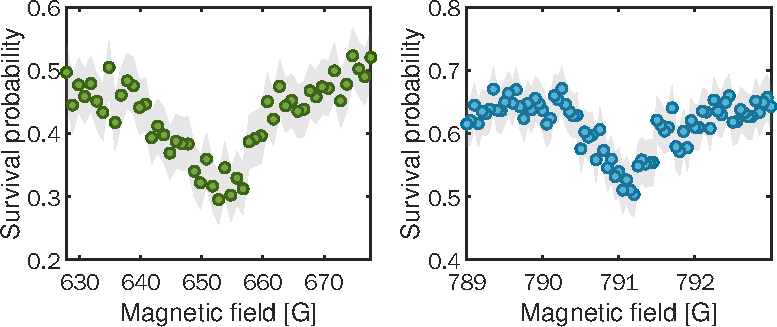
\includegraphics[width=10cm]{fb.pdf}\\
      \vspace{0.5cm}
    \end{center}
  }
  \only<3->{
    \begin{center}
      \begin{tabular}{|c|p{1.9cm}|p{1.9cm}|}
        \hline
        &$s$-wave&$p$-wave\\\hline
        Predicted {\tiny (based on interaction shift)\footnote{In collaboration with Bo Gao}}&$663$ G&$799$ G\\\hline
        Measured&$652(3)$ G&$791.2(2)$ G\\\hline
      \end{tabular}
    \end{center}
  }
\end{frame}

\begin{frame}{Conclusion}
  \begin{center}
    \begin{itemize}
    \item Interaction shift of Na and Cs
    \item Feshbach resonance Na(1,-1) Cs(3,-3)
    \end{itemize}
    \vspace{1cm}
    \visible<2->{
      {\usebeamerfont{frametitle}\usebeamercolor[fg]{frametitle}{Next step}}
      \begin{itemize}
      \item Make Feshbach molecules
      \item Optical molecule formation taking advantage of the large scattering length
      \end{itemize}
      \vspace{1cm}
    }
    \visible<3->{
      Thank you for your attention.\\
      % Poster
      Poster S01.00155 (Thursday afternoon)
    }
  \end{center}
\end{frame}

\end{document}
